\SourceLeaf{259}%
\[
\frac{R}{\rho}\alpha = \frac{R}{\lambda} F(a, \rho-\beta)
\]
oder]
\[
\tag*{2)} \alpha = \frac{\rho}{\lambda} F(a, \rho-\beta).
\]

[Ebenso ergibt das Viereck $BHGC$:]
\[
\tag*{3)} \beta = \frac{\rho}{\lambda} F(b, \rho-\alpha).
\]

\Needspace{24\baselineskip}
\begin{center}\begin{minipage}{\linewidth}\centering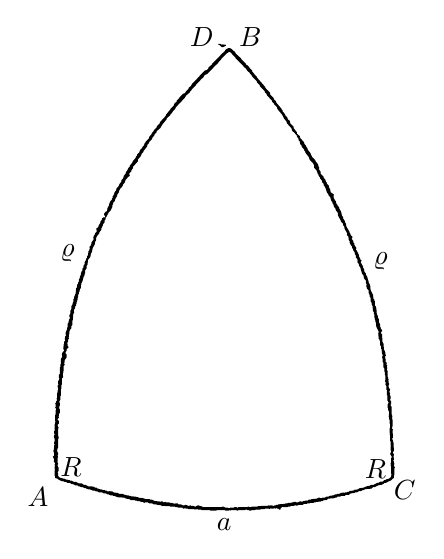
\begin{tikzpicture}[x=0.00604333cm,y=-0.00604333cm]
\fill[even odd rule] (455,69) -- (451,71) -- (448,74) -- (448,75) -- (438,84) -- (438,85) -- (421,102) -- (421,103) -- (413,110) -- (413,112) -- (410,115) -- (406,116) -- (394,128) -- (394,129) -- (390,132) -- (390,133) -- (379,144) -- (376,149) -- (372,152) -- (371,155) -- (365,161) -- (365,162) -- (363,164) -- (360,165) -- (352,173) -- (352,174) -- (346,180) -- (346,182) -- (342,185) -- (340,190) -- (333,197) -- (333,198) -- (324,209) -- (323,212) -- (311,225) -- (311,227) -- (305,233) -- (304,236) -- (299,241) -- (297,245) -- (294,248) -- (293,251) -- (289,255) -- (288,259) -- (281,266) -- (281,267) -- (279,269) -- (278,273) -- (275,276) -- (273,280) -- (269,284) -- (268,288) -- (263,293) -- (263,295) -- (261,297) -- (260,300) -- (254,307) -- (253,310) -- (248,316) -- (248,318) -- (245,321) -- (242,327) -- (240,329) -- (239,333) -- (235,338) -- (235,340) -- (233,344) -- (230,347) -- (230,350) -- (226,355) -- (224,360) -- (220,364) -- (219,368) -- (216,372) -- (214,378) -- (212,380) -- (212,384) -- (210,386) -- (210,388) -- (207,391) -- (205,395) -- (204,400) -- (201,405) -- (200,411) -- (198,413) -- (197,413) -- (194,417) -- (194,420) -- (196,422) -- (196,424) -- (195,425) -- (192,425) -- (189,428) -- (189,430) -- (186,434) -- (186,436) -- (182,443) -- (182,445) -- (177,449) -- (178,451) -- (178,455) -- (175,458) -- (175,460) -- (172,464) -- (172,466) -- (171,467) -- (172,471) -- (167,478) -- (167,481) -- (165,485) -- (163,487) -- (164,490) -- (163,491) -- (163,494) -- (161,496) -- (160,504) -- (158,507) -- (158,510) -- (156,512) -- (156,514) -- (153,519) -- (153,523) -- (151,525) -- (150,531) -- (148,533) -- (148,537) -- (146,539) -- (146,541) -- (145,542) -- (145,546) -- (143,549) -- (143,552) -- (141,555) -- (141,560) -- (139,562) -- (139,564) -- (137,567) -- (137,572) -- (135,574) -- (134,585) -- (131,592) -- (131,595) -- (129,597) -- (129,603) -- (128,604) -- (127,609) -- (125,611) -- (125,617) -- (123,621) -- (123,627) -- (121,630) -- (121,634) -- (122,635) -- (122,637) -- (120,640) -- (119,646) -- (117,649) -- (117,656) -- (116,657) -- (116,660) -- (113,667) -- (113,671) -- (114,673) -- (112,675) -- (112,679) -- (111,680) -- (112,684) -- (110,686) -- (110,691) -- (109,692) -- (109,696) -- (108,697) -- (108,702) -- (110,704) -- (110,705) -- (107,708) -- (105,712) -- (106,718) -- (103,722) -- (103,733) -- (102,734) -- (102,739) -- (101,740) -- (101,753) -- (99,756) -- (99,762) -- (100,764) -- (97,770) -- (97,774) -- (98,776) -- (96,779) -- (96,782) -- (97,783) -- (97,788) -- (96,789) -- (96,793) -- (95,794) -- (95,804) -- (94,805) -- (95,809) -- (93,812) -- (93,814) -- (91,816) -- (92,818) -- (92,823) -- (91,825) -- (93,827) -- (93,829) -- (92,830) -- (92,839) -- (91,840) -- (91,853) -- (92,855) -- (91,856) -- (91,859) -- (90,860) -- (90,873) -- (89,874) -- (89,879) -- (90,881) -- (88,885) -- (89,889) -- (90,890) -- (90,896) -- (89,897) -- (89,901) -- (90,903) -- (89,904) -- (89,909) -- (88,910) -- (88,914) -- (87,915) -- (88,919) -- (89,920) -- (89,925) -- (86,928) -- (89,933) -- (88,938) -- (91,941) -- (91,943) -- (90,944) -- (90,946) -- (91,947) -- (90,949) -- (90,953) -- (91,954) -- (90,956) -- (90,968) -- (91,969) -- (91,972) -- (92,973) -- (96,974) -- (98,976) -- (104,979) -- (110,980) -- (111,981) -- (114,981) -- (117,983) -- (122,983) -- (125,985) -- (130,986) -- (133,988) -- (138,988) -- (140,990) -- (142,990) -- (146,992) -- (149,992) -- (153,994) -- (156,994) -- (158,996) -- (166,997) -- (170,999) -- (174,999) -- (177,1001) -- (180,1001) -- (183,1003) -- (190,1003) -- (193,1005) -- (198,1005) -- (201,1007) -- (203,1007) -- (207,1009) -- (212,1009) -- (213,1010) -- (215,1010) -- (222,1013) -- (237,1014) -- (240,1016) -- (247,1017) -- (250,1019) -- (258,1019) -- (259,1020) -- (262,1020) -- (263,1021) -- (268,1021) -- (272,1023) -- (276,1023) -- (278,1025) -- (280,1024) -- (286,1024) -- (289,1026) -- (295,1026) -- (298,1028) -- (304,1028) -- (305,1029) -- (314,1030) -- (316,1032) -- (318,1031) -- (322,1031) -- (323,1032) -- (332,1032) -- (333,1033) -- (343,1033) -- (344,1034) -- (348,1034) -- (349,1035) -- (358,1035) -- (360,1037) -- (365,1036) -- (366,1037) -- (370,1037) -- (371,1038) -- (383,1038) -- (384,1039) -- (390,1038) -- (391,1039) -- (398,1039) -- (399,1040) -- (416,1040) -- (417,1041) -- (430,1041) -- (431,1040) -- (448,1040) -- (449,1041) -- (456,1041) -- (457,1040) -- (459,1041) -- (461,1040) -- (472,1040) -- (473,1041) -- (475,1041) -- (476,1040) -- (490,1040) -- (491,1039) -- (494,1039) -- (495,1040) -- (498,1040) -- (499,1041) -- (503,1041) -- (504,1040) -- (511,1040) -- (512,1039) -- (522,1039) -- (523,1038) -- (531,1038) -- (532,1037) -- (540,1037) -- (542,1038) -- (544,1036) -- (546,1037) -- (550,1037) -- (551,1036) -- (554,1037) -- (555,1036) -- (557,1036) -- (558,1037) -- (560,1037) -- (562,1039) -- (564,1039) -- (565,1038) -- (565,1036) -- (569,1033) -- (571,1034) -- (579,1034) -- (580,1033) -- (584,1033) -- (587,1031) -- (593,1031) -- (594,1030) -- (597,1030) -- (599,1031) -- (603,1029) -- (611,1029) -- (615,1027) -- (620,1027) -- (621,1026) -- (626,1026) -- (627,1025) -- (634,1025) -- (635,1024) -- (638,1024) -- (639,1023) -- (649,1022) -- (650,1021) -- (653,1021) -- (656,1019) -- (661,1019) -- (665,1016) -- (678,1015) -- (679,1014) -- (682,1014) -- (684,1012) -- (690,1012) -- (692,1010) -- (700,1010) -- (702,1008) -- (708,1008) -- (712,1005) -- (720,1004) -- (721,1003) -- (725,1003) -- (730,1000) -- (734,1000) -- (737,998) -- (739,998) -- (743,996) -- (756,995) -- (759,992) -- (762,992) -- (770,988) -- (777,987) -- (781,985) -- (783,983) -- (786,983) -- (793,979) -- (795,979) -- (803,972) -- (803,967) -- (804,966) -- (804,953) -- (805,951) -- (803,947) -- (804,942) -- (803,941) -- (803,938) -- (802,937) -- (802,935) -- (803,934) -- (803,930) -- (802,929) -- (803,923) -- (801,920) -- (801,918) -- (803,916) -- (802,897) -- (801,896) -- (801,893) -- (799,891) -- (799,890) -- (801,888) -- (801,880) -- (800,879) -- (800,873) -- (801,871) -- (799,869) -- (799,865) -- (800,864) -- (800,850) -- (799,849) -- (799,846) -- (800,844) -- (799,843) -- (799,840) -- (798,839) -- (798,823) -- (796,820) -- (796,818) -- (797,817) -- (797,811) -- (795,809) -- (795,807) -- (796,806) -- (796,800) -- (794,798) -- (795,794) -- (793,792) -- (795,787) -- (792,782) -- (792,777) -- (793,776) -- (793,774) -- (792,773) -- (792,770) -- (791,769) -- (792,765) -- (791,764) -- (791,761) -- (790,760) -- (790,748) -- (788,745) -- (788,743) -- (789,742) -- (788,738) -- (789,736) -- (787,734) -- (788,731) -- (785,728) -- (786,724) -- (785,723) -- (785,720) -- (784,718) -- (786,716) -- (786,714) -- (785,713) -- (785,709) -- (784,708) -- (784,706) -- (782,703) -- (781,690) -- (779,687) -- (778,671) -- (776,669) -- (776,666) -- (778,664) -- (778,662) -- (775,658) -- (775,656) -- (774,655) -- (774,649) -- (772,647) -- (771,638) -- (769,635) -- (769,632) -- (767,628) -- (766,615) -- (765,614) -- (765,612) -- (763,610) -- (763,601) -- (762,600) -- (762,598) -- (760,596) -- (759,588) -- (754,578) -- (753,567) -- (750,562) -- (750,559) -- (749,558) -- (747,550) -- (744,545) -- (744,543) -- (741,539) -- (740,533) -- (738,531) -- (738,528) -- (733,519) -- (735,516) -- (732,513) -- (732,511) -- (730,508) -- (729,503) -- (725,495) -- (723,493) -- (724,489) -- (720,483) -- (720,480) -- (718,478) -- (718,475) -- (714,470) -- (716,466) -- (712,462) -- (712,460) -- (710,458) -- (710,456) -- (703,444) -- (702,438) -- (700,435) -- (700,433) -- (696,427) -- (696,424) -- (694,422) -- (692,413) -- (688,406) -- (688,404) -- (685,401) -- (684,398) -- (682,396) -- (681,391) -- (679,389) -- (676,383) -- (676,379) -- (677,377) -- (670,372) -- (669,366) -- (667,363) -- (666,358) -- (662,354) -- (662,352) -- (660,350) -- (659,346) -- (655,341) -- (655,339) -- (649,333) -- (649,329) -- (646,325) -- (646,320) -- (644,317) -- (644,315) -- (642,311) -- (639,308) -- (637,304) -- (631,298) -- (627,289) -- (622,283) -- (621,279) -- (619,277) -- (618,274) -- (615,271) -- (614,267) -- (606,258) -- (605,254) -- (599,249) -- (599,246) -- (592,237) -- (592,234) -- (585,227) -- (585,224) -- (584,222) -- (580,219) -- (579,215) -- (575,211) -- (574,208) -- (569,202) -- (569,200) -- (567,198) -- (567,197) -- (556,184) -- (555,181) -- (551,177) -- (550,174) -- (544,168) -- (543,166) -- (543,163) -- (534,154) -- (531,149) -- (516,132) -- (514,128) -- (510,125) -- (510,124) -- (505,118) -- (505,116) -- (499,110) -- (499,109) -- (495,105) -- (494,105) -- (492,103) -- (492,102) -- (482,92) -- (482,91) -- (471,81) -- (468,76) -- (467,76) -- (462,71) -- (458,69) -- cycle
(458,77) -- (462,80) -- (462,81) -- (470,89) -- (470,90) -- (487,107) -- (487,108) -- (492,112) -- (495,117) -- (500,121) -- (500,122) -- (503,125) -- (506,130) -- (515,139) -- (515,141) -- (521,147) -- (521,149) -- (531,159) -- (532,162) -- (535,165) -- (536,168) -- (547,180) -- (547,182) -- (551,186) -- (551,187) -- (557,193) -- (558,197) -- (568,209) -- (572,217) -- (577,223) -- (578,227) -- (588,238) -- (589,243) -- (591,245) -- (592,245) -- (599,253) -- (599,255) -- (602,259) -- (603,263) -- (605,265) -- (606,271) -- (609,274) -- (609,276) -- (614,282) -- (615,285) -- (617,287) -- (617,289) -- (624,298) -- (626,304) -- (633,311) -- (635,315) -- (635,320) -- (641,327) -- (641,329) -- (642,330) -- (642,332) -- (644,334) -- (644,336) -- (646,338) -- (646,339) -- (648,341) -- (648,343) -- (652,348) -- (652,351) -- (655,354) -- (655,357) -- (657,359) -- (660,365) -- (662,372) -- (665,376) -- (666,379) -- (669,382) -- (671,389) -- (674,394) -- (674,396) -- (676,398) -- (676,400) -- (678,404) -- (680,406) -- (681,410) -- (685,415) -- (685,420) -- (693,435) -- (696,438) -- (696,441) -- (698,443) -- (699,445) -- (699,448) -- (705,459) -- (704,462) -- (707,465) -- (707,467) -- (708,468) -- (708,472) -- (710,475) -- (710,478) -- (713,484) -- (715,486) -- (715,489) -- (717,491) -- (718,495) -- (720,497) -- (721,502) -- (723,505) -- (723,509) -- (726,512) -- (726,515) -- (727,516) -- (726,519) -- (728,521) -- (730,525) -- (730,527) -- (732,529) -- (736,543) -- (739,547) -- (740,553) -- (745,559) -- (744,561) -- (744,563) -- (746,566) -- (745,568) -- (745,571) -- (746,572) -- (746,574) -- (750,578) -- (750,584) -- (752,588) -- (752,591) -- (754,594) -- (754,601) -- (756,604) -- (756,607) -- (758,611) -- (759,622) -- (761,624) -- (761,628) -- (762,629) -- (762,636) -- (763,637) -- (763,640) -- (764,641) -- (764,644) -- (765,645) -- (766,655) -- (771,665) -- (771,667) -- (770,668) -- (771,680) -- (773,682) -- (773,684) -- (774,685) -- (774,693) -- (776,696) -- (776,701) -- (777,702) -- (778,712) -- (779,713) -- (779,717) -- (778,718) -- (778,720) -- (780,722) -- (779,724) -- (779,728) -- (781,731) -- (781,740) -- (783,743) -- (783,749) -- (784,750) -- (784,756) -- (785,757) -- (785,767) -- (784,769) -- (786,772) -- (785,776) -- (787,779) -- (787,787) -- (789,789) -- (788,791) -- (788,798) -- (789,799) -- (789,809) -- (792,814) -- (790,818) -- (790,825) -- (791,826) -- (791,830) -- (793,834) -- (792,844) -- (793,845) -- (793,849) -- (794,850) -- (794,858) -- (795,859) -- (795,867) -- (794,868) -- (794,878) -- (795,880) -- (794,882) -- (795,883) -- (795,895) -- (796,896) -- (796,904) -- (797,905) -- (796,907) -- (796,914) -- (797,915) -- (797,918) -- (795,922) -- (798,927) -- (798,930) -- (797,931) -- (797,940) -- (796,941) -- (796,943) -- (797,944) -- (796,946) -- (797,948) -- (797,963) -- (798,964) -- (797,970) -- (794,973) -- (790,975) -- (788,975) -- (785,977) -- (783,977) -- (780,980) -- (775,980) -- (770,983) -- (768,983) -- (760,987) -- (755,987) -- (752,989) -- (746,990) -- (739,993) -- (731,994) -- (726,997) -- (721,997) -- (718,999) -- (710,1000) -- (708,1002) -- (705,1002) -- (704,1003) -- (700,1003) -- (699,1004) -- (696,1003) -- (695,1004) -- (692,1004) -- (688,1006) -- (684,1006) -- (683,1007) -- (680,1007) -- (676,1009) -- (669,1010) -- (665,1012) -- (661,1012) -- (658,1014) -- (653,1014) -- (652,1015) -- (648,1015) -- (647,1014) -- (645,1014) -- (641,1016) -- (630,1017) -- (629,1018) -- (624,1018) -- (622,1020) -- (616,1020) -- (615,1021) -- (612,1021) -- (610,1023) -- (608,1022) -- (605,1022) -- (601,1024) -- (598,1024) -- (597,1023) -- (592,1023) -- (591,1024) -- (588,1024) -- (587,1025) -- (580,1025) -- (579,1026) -- (575,1026) -- (574,1027) -- (560,1028) -- (559,1029) -- (556,1029) -- (555,1030) -- (552,1030) -- (551,1031) -- (548,1031) -- (547,1030) -- (544,1030) -- (542,1031) -- (541,1030) -- (539,1030) -- (538,1031) -- (524,1031) -- (523,1032) -- (517,1032) -- (516,1033) -- (504,1033) -- (503,1034) -- (499,1034) -- (498,1033) -- (496,1033) -- (495,1034) -- (476,1034) -- (475,1035) -- (473,1035) -- (472,1034) -- (468,1034) -- (467,1035) -- (459,1035) -- (458,1036) -- (455,1036) -- (454,1035) -- (449,1035) -- (445,1033) -- (442,1033) -- (441,1034) -- (402,1034) -- (398,1032) -- (395,1032) -- (393,1030) -- (391,1030) -- (385,1033) -- (381,1031) -- (376,1031) -- (375,1030) -- (373,1031) -- (370,1031) -- (366,1029) -- (364,1029) -- (363,1030) -- (359,1030) -- (355,1028) -- (350,1028) -- (348,1026) -- (344,1026) -- (342,1027) -- (341,1026) -- (338,1026) -- (337,1025) -- (332,1025) -- (331,1024) -- (324,1024) -- (323,1023) -- (319,1024) -- (317,1022) -- (313,1022) -- (312,1023) -- (310,1022) -- (305,1022) -- (304,1021) -- (300,1021) -- (294,1018) -- (290,1018) -- (289,1017) -- (281,1017) -- (280,1016) -- (277,1016) -- (276,1015) -- (266,1014) -- (265,1013) -- (262,1013) -- (261,1012) -- (250,1011) -- (249,1010) -- (246,1010) -- (245,1009) -- (241,1009) -- (240,1008) -- (237,1008) -- (233,1006) -- (226,1006) -- (222,1004) -- (214,1003) -- (211,1001) -- (207,1001) -- (206,1000) -- (204,1001) -- (201,1001) -- (199,999) -- (196,999) -- (195,998) -- (191,998) -- (190,997) -- (183,996) -- (182,995) -- (180,995) -- (178,993) -- (175,993) -- (172,991) -- (169,991) -- (168,990) -- (160,990) -- (155,987) -- (151,987) -- (147,984) -- (141,984) -- (135,981) -- (131,981) -- (125,978) -- (122,978) -- (121,977) -- (118,977) -- (117,976) -- (114,976) -- (110,974) -- (107,974) -- (106,973) -- (101,972) -- (97,968) -- (97,962) -- (96,961) -- (96,960) -- (98,958) -- (98,951) -- (96,947) -- (96,945) -- (97,944) -- (97,942) -- (96,941) -- (96,930) -- (97,929) -- (96,925) -- (97,924) -- (97,920) -- (95,916) -- (96,910) -- (97,909) -- (97,891) -- (98,890) -- (98,885) -- (97,884) -- (97,869) -- (98,868) -- (98,866) -- (97,865) -- (96,861) -- (99,858) -- (99,853) -- (96,850) -- (96,849) -- (99,846) -- (98,843) -- (99,842) -- (99,838) -- (101,835) -- (101,829) -- (99,825) -- (100,824) -- (100,821) -- (101,820) -- (101,815) -- (100,814) -- (100,811) -- (102,808) -- (102,800) -- (103,799) -- (103,786) -- (104,785) -- (104,777) -- (105,776) -- (105,764) -- (108,760) -- (107,758) -- (107,752) -- (108,751) -- (108,748) -- (109,747) -- (109,737) -- (111,735) -- (111,733) -- (110,732) -- (110,730) -- (111,729) -- (111,725) -- (115,719) -- (115,713) -- (113,711) -- (113,708) -- (115,705) -- (115,702) -- (119,698) -- (119,697) -- (117,695) -- (117,691) -- (116,689) -- (118,686) -- (118,682) -- (120,680) -- (119,677) -- (120,676) -- (120,671) -- (121,670) -- (121,664) -- (123,660) -- (125,658) -- (125,653) -- (127,651) -- (127,642) -- (128,641) -- (129,628) -- (131,625) -- (130,620) -- (133,615) -- (133,612) -- (135,610) -- (135,607) -- (136,606) -- (136,603) -- (137,602) -- (137,599) -- (138,598) -- (138,594) -- (139,593) -- (139,588) -- (141,585) -- (141,582) -- (142,581) -- (143,576) -- (145,573) -- (145,567) -- (146,566) -- (146,563) -- (148,560) -- (151,549) -- (153,546) -- (153,543) -- (154,542) -- (154,536) -- (157,532) -- (157,527) -- (159,524) -- (160,514) -- (165,508) -- (166,501) -- (168,498) -- (170,489) -- (174,482) -- (175,476) -- (177,473) -- (177,468) -- (179,464) -- (184,458) -- (184,456) -- (188,451) -- (188,448) -- (191,442) -- (191,440) -- (195,435) -- (195,431) -- (197,429) -- (197,425) -- (200,422) -- (200,420) -- (202,418) -- (203,415) -- (207,411) -- (211,403) -- (211,399) -- (213,397) -- (213,394) -- (216,391) -- (217,387) -- (221,380) -- (222,376) -- (225,372) -- (225,370) -- (228,364) -- (232,360) -- (234,355) -- (237,352) -- (239,346) -- (242,343) -- (242,342) -- (248,337) -- (247,335) -- (247,332) -- (251,328) -- (251,326) -- (254,322) -- (255,318) -- (264,308) -- (265,306) -- (265,303) -- (271,296) -- (273,291) -- (276,288) -- (277,285) -- (284,276) -- (285,272) -- (287,270) -- (289,266) -- (294,261) -- (296,256) -- (299,253) -- (300,250) -- (304,246) -- (304,244) -- (312,237) -- (316,230) -- (325,219) -- (325,217) -- (333,210) -- (333,209) -- (336,206) -- (339,201) -- (343,197) -- (345,193) -- (363,174) -- (366,169) -- (374,162) -- (374,161) -- (378,157) -- (378,156) -- (387,147) -- (387,146) -- (396,137) -- (396,136) -- (403,130) -- (404,127) -- (406,125) -- (410,124) -- (424,110) -- (424,109) -- (434,100) -- (434,99) -- (440,93) -- (440,92) -- (453,79) -- (454,79) -- (456,77) -- cycle
(434,60) -- (434,62) -- (437,63) -- (441,67) -- (444,67) -- (450,64) -- (449,62) -- (445,62) -- (444,61) -- (441,62) -- (438,60) -- cycle;
\node[inner sep=0pt] at (399,46) {$D$};
\node[inner sep=0pt] at (501,46) {$B$};
\node[inner sep=0pt] at (117,500) {$\varrho$};
\node[inner sep=0pt] at (775,517) {$\varrho$};
\node[inner sep=0pt] at (124,950) {$R$};
\node[inner sep=0pt] at (764,954) {$R$};
\node[inner sep=0pt] at (55,1013) {$A$};
\node[inner sep=0pt] at (826,997) {$C$};
\node[inner sep=0pt] at (446,1071) {$a$};
\end{tikzpicture}
\\[3pt]Fig. 4.\end{minipage}\end{center}

[Ferner ist nach Fig. 4:]
\[
\tag*{4)} a\frac{\lambda}{\rho} = F(a, \rho),
\]

[und für unendlich kleine $a$ ist
\[
F(a,\rho) = af\rho = a\frac{\lambda}{\rho},
\]
also]
\[
\tag*{5)} \frac{\lambda}{\rho} = f\rho.
\]

Für unendlich kleine $a$ ist
\[
\alpha = \frac{\rho}{\lambda}\cdot af(\rho-\beta)
\]
also selbst unendlich klein, daher dann aus 3) $\beta$ unendlich wenig von
\[
\frac{\rho}{\lambda} F(b,\rho)
\]
d.\,i. von $b$ verschieden.

\Needspace{25\baselineskip}
Ferner [ergibt Fig. 5] die vollständige allgemeine Differentialgleichung

\begin{center}\begin{minipage}{\linewidth}\centering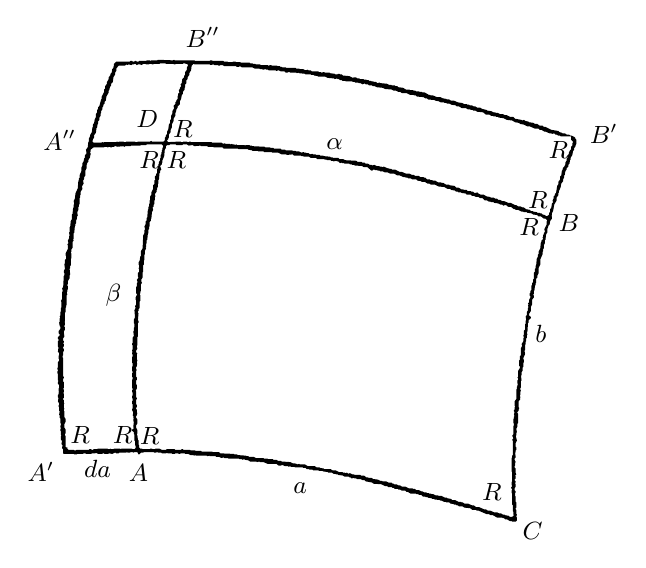
\begin{tikzpicture}[x=0.00742115cm,y=-0.00742115cm]
\fill[even odd rule] (184,73) -- (180,77) -- (180,81) -- (179,82) -- (179,84) -- (177,86) -- (176,92) -- (174,94) -- (174,96) -- (171,100) -- (171,103) -- (168,108) -- (168,111) -- (165,115) -- (165,119) -- (163,121) -- (163,125) -- (159,133) -- (159,137) -- (158,138) -- (155,149) -- (153,151) -- (153,153) -- (151,157) -- (151,160) -- (149,163) -- (149,168) -- (147,172) -- (146,178) -- (144,181) -- (144,185) -- (143,186) -- (142,194) -- (139,199) -- (139,201) -- (137,205) -- (137,210) -- (136,211) -- (135,220) -- (132,224) -- (133,230) -- (130,234) -- (130,238) -- (129,239) -- (128,244) -- (126,247) -- (126,251) -- (124,255) -- (124,261) -- (121,268) -- (121,272) -- (120,273) -- (120,276) -- (119,277) -- (118,290) -- (114,299) -- (113,308) -- (111,312) -- (112,317) -- (111,318) -- (111,323) -- (110,324) -- (109,334) -- (108,335) -- (108,343) -- (106,346) -- (105,356) -- (104,357) -- (104,365) -- (103,366) -- (104,371) -- (103,372) -- (103,376) -- (101,380) -- (102,384) -- (100,386) -- (101,388) -- (101,394) -- (97,402) -- (97,405) -- (98,406) -- (98,411) -- (96,413) -- (96,419) -- (95,420) -- (96,428) -- (94,432) -- (94,434) -- (95,435) -- (95,439) -- (94,440) -- (93,459) -- (91,462) -- (92,464) -- (92,467) -- (91,468) -- (91,480) -- (89,483) -- (90,485) -- (90,494) -- (89,495) -- (89,501) -- (88,502) -- (88,508) -- (87,509) -- (88,512) -- (87,513) -- (87,519) -- (86,520) -- (87,526) -- (88,527) -- (88,531) -- (85,535) -- (85,538) -- (87,540) -- (87,542) -- (84,545) -- (84,548) -- (85,549) -- (85,551) -- (84,552) -- (84,561) -- (85,562) -- (84,570) -- (86,572) -- (86,576) -- (85,577) -- (85,582) -- (86,583) -- (86,585) -- (84,588) -- (84,597) -- (83,598) -- (83,600) -- (84,601) -- (84,603) -- (83,604) -- (83,607) -- (84,608) -- (84,619) -- (85,620) -- (84,622) -- (84,625) -- (86,627) -- (86,632) -- (85,633) -- (85,637) -- (86,639) -- (85,640) -- (85,643) -- (84,644) -- (84,648) -- (85,649) -- (84,655) -- (86,659) -- (86,661) -- (85,662) -- (85,664) -- (86,665) -- (86,671) -- (87,672) -- (86,678) -- (87,679) -- (87,683) -- (88,684) -- (88,692) -- (89,693) -- (89,696) -- (88,697) -- (89,702) -- (88,703) -- (88,705) -- (89,706) -- (89,712) -- (90,713) -- (89,715) -- (89,720) -- (91,723) -- (90,728) -- (92,730) -- (91,735) -- (93,737) -- (93,744) -- (94,745) -- (111,745) -- (112,746) -- (116,746) -- (117,745) -- (127,745) -- (128,744) -- (131,744) -- (132,745) -- (141,745) -- (142,744) -- (148,744) -- (149,743) -- (153,745) -- (160,745) -- (161,744) -- (163,744) -- (164,745) -- (170,745) -- (171,744) -- (177,745) -- (181,743) -- (183,743) -- (184,744) -- (188,744) -- (189,743) -- (201,743) -- (202,742) -- (204,743) -- (207,743) -- (208,742) -- (212,742) -- (213,743) -- (215,742) -- (220,742) -- (222,746) -- (223,746) -- (226,743) -- (230,743) -- (231,742) -- (248,742) -- (249,743) -- (255,742) -- (256,743) -- (261,743) -- (262,744) -- (269,744) -- (271,743) -- (272,744) -- (279,744) -- (280,745) -- (284,745) -- (285,744) -- (290,744) -- (291,745) -- (293,745) -- (294,744) -- (301,744) -- (302,745) -- (307,745) -- (311,747) -- (316,747) -- (317,748) -- (319,747) -- (321,748) -- (339,748) -- (340,749) -- (343,748) -- (344,749) -- (354,749) -- (355,750) -- (360,750) -- (364,752) -- (368,751) -- (369,752) -- (375,752) -- (376,753) -- (394,753) -- (395,754) -- (399,754) -- (400,755) -- (403,754) -- (404,755) -- (410,756) -- (413,758) -- (424,758) -- (425,759) -- (429,758) -- (430,759) -- (436,759) -- (443,762) -- (458,762) -- (462,765) -- (466,765) -- (467,764) -- (469,764) -- (473,766) -- (478,766) -- (479,767) -- (482,766) -- (483,767) -- (489,767) -- (490,768) -- (503,768) -- (504,769) -- (508,769) -- (510,771) -- (514,771) -- (515,772) -- (520,772) -- (521,773) -- (530,773) -- (531,774) -- (537,774) -- (538,775) -- (546,776) -- (547,777) -- (553,777) -- (556,779) -- (559,779) -- (560,780) -- (563,780) -- (564,781) -- (572,782) -- (575,784) -- (582,784) -- (583,785) -- (585,785) -- (587,787) -- (591,786) -- (592,787) -- (595,787) -- (596,788) -- (602,788) -- (606,790) -- (609,790) -- (611,792) -- (622,794) -- (624,796) -- (638,797) -- (644,800) -- (648,800) -- (650,802) -- (656,802) -- (657,803) -- (659,803) -- (661,805) -- (666,805) -- (667,806) -- (670,806) -- (673,808) -- (679,808) -- (681,810) -- (683,810) -- (688,813) -- (697,813) -- (698,814) -- (701,814) -- (702,815) -- (706,815) -- (709,818) -- (713,818) -- (714,819) -- (717,819) -- (718,820) -- (724,821) -- (725,822) -- (728,822) -- (729,823) -- (738,824) -- (739,825) -- (741,825) -- (745,827) -- (748,827) -- (749,828) -- (754,828) -- (756,830) -- (762,831) -- (763,832) -- (766,832) -- (767,833) -- (769,833) -- (771,835) -- (777,835) -- (780,837) -- (790,838) -- (794,841) -- (800,841) -- (801,842) -- (804,842) -- (818,848) -- (822,848) -- (825,850) -- (829,850) -- (836,854) -- (845,854) -- (846,855) -- (848,855) -- (850,857) -- (853,857) -- (858,860) -- (861,860) -- (862,861) -- (868,861) -- (870,859) -- (870,854) -- (869,853) -- (870,849) -- (869,848) -- (869,841) -- (868,840) -- (868,838) -- (869,837) -- (869,828) -- (868,827) -- (868,818) -- (867,817) -- (867,812) -- (868,811) -- (868,809) -- (866,807) -- (866,804) -- (868,801) -- (868,797) -- (867,796) -- (868,792) -- (866,790) -- (866,789) -- (868,787) -- (868,784) -- (867,782) -- (869,780) -- (868,778) -- (868,770) -- (866,768) -- (866,766) -- (867,765) -- (867,760) -- (868,759) -- (866,755) -- (866,753) -- (868,751) -- (867,743) -- (868,742) -- (868,739) -- (869,738) -- (869,734) -- (868,733) -- (868,726) -- (870,722) -- (868,714) -- (869,713) -- (869,709) -- (870,708) -- (869,702) -- (871,698) -- (871,693) -- (872,692) -- (872,676) -- (871,675) -- (871,673) -- (873,671) -- (873,669) -- (874,668) -- (874,666) -- (873,665) -- (873,655) -- (876,651) -- (875,650) -- (876,648) -- (875,645) -- (876,644) -- (876,638) -- (877,637) -- (876,635) -- (876,632) -- (877,631) -- (877,620) -- (878,619) -- (877,611) -- (878,610) -- (878,605) -- (880,602) -- (880,597) -- (881,596) -- (881,589) -- (882,588) -- (882,584) -- (881,583) -- (881,581) -- (884,574) -- (883,568) -- (884,567) -- (884,558) -- (885,557) -- (885,553) -- (886,552) -- (886,547) -- (887,546) -- (887,542) -- (888,541) -- (887,537) -- (888,536) -- (889,521) -- (890,520) -- (890,516) -- (893,513) -- (894,513) -- (894,510) -- (893,510) -- (891,508) -- (891,505) -- (894,500) -- (894,493) -- (896,489) -- (896,481) -- (899,477) -- (899,474) -- (898,472) -- (899,471) -- (899,466) -- (900,465) -- (901,457) -- (902,456) -- (902,453) -- (903,452) -- (903,445) -- (905,443) -- (905,440) -- (907,436) -- (907,427) -- (910,421) -- (910,412) -- (914,403) -- (914,399) -- (915,398) -- (915,394) -- (916,393) -- (916,388) -- (918,384) -- (918,379) -- (919,378) -- (920,369) -- (922,366) -- (922,359) -- (923,358) -- (924,354) -- (926,352) -- (927,346) -- (930,342) -- (930,339) -- (929,337) -- (930,336) -- (930,333) -- (932,329) -- (934,318) -- (938,311) -- (938,306) -- (941,302) -- (941,298) -- (942,297) -- (942,295) -- (945,288) -- (946,282) -- (949,278) -- (949,275) -- (951,271) -- (951,268) -- (952,267) -- (953,261) -- (955,258) -- (955,256) -- (958,253) -- (958,250) -- (960,248) -- (961,242) -- (962,241) -- (962,238) -- (965,233) -- (966,227) -- (968,224) -- (968,221) -- (970,219) -- (971,215) -- (972,214) -- (972,207) -- (970,205) -- (970,204) -- (968,202) -- (964,200) -- (962,200) -- (959,198) -- (955,198) -- (952,196) -- (948,196) -- (947,195) -- (943,194) -- (941,192) -- (929,190) -- (919,185) -- (916,185) -- (914,183) -- (909,183) -- (905,180) -- (901,180) -- (898,178) -- (891,177) -- (890,176) -- (885,175) -- (882,173) -- (879,174) -- (878,173) -- (867,171) -- (864,168) -- (859,168) -- (853,165) -- (850,165) -- (846,163) -- (841,163) -- (837,161) -- (834,161) -- (833,160) -- (830,160) -- (826,158) -- (819,157) -- (818,156) -- (810,154) -- (807,152) -- (802,152) -- (799,150) -- (796,150) -- (793,148) -- (789,148) -- (788,147) -- (785,147) -- (784,146) -- (780,146) -- (776,144) -- (769,143) -- (762,140) -- (757,140) -- (754,138) -- (750,138) -- (749,137) -- (743,136) -- (739,134) -- (733,134) -- (726,131) -- (722,131) -- (721,130) -- (719,130) -- (712,126) -- (708,126) -- (707,125) -- (703,125) -- (702,124) -- (697,124) -- (696,123) -- (693,123) -- (692,122) -- (687,122) -- (686,121) -- (680,121) -- (675,118) -- (667,117) -- (665,115) -- (662,115) -- (661,114) -- (656,114) -- (655,113) -- (651,113) -- (647,111) -- (636,110) -- (635,109) -- (631,110) -- (629,108) -- (625,108) -- (624,107) -- (621,107) -- (620,106) -- (617,106) -- (616,105) -- (613,105) -- (612,104) -- (608,104) -- (607,103) -- (601,103) -- (600,102) -- (597,102) -- (594,100) -- (591,100) -- (589,101) -- (583,98) -- (572,97) -- (570,95) -- (567,95) -- (566,94) -- (564,94) -- (563,95) -- (559,95) -- (558,94) -- (550,93) -- (549,92) -- (541,92) -- (540,91) -- (535,92) -- (534,91) -- (531,91) -- (530,90) -- (519,90) -- (517,88) -- (513,88) -- (512,87) -- (508,88) -- (504,86) -- (498,86) -- (497,85) -- (492,85) -- (491,84) -- (475,84) -- (474,83) -- (468,83) -- (467,82) -- (465,82) -- (464,81) -- (460,81) -- (459,80) -- (450,80) -- (449,79) -- (447,79) -- (446,80) -- (444,80) -- (443,79) -- (431,79) -- (430,78) -- (423,78) -- (422,77) -- (418,77) -- (417,76) -- (413,76) -- (412,75) -- (397,75) -- (396,74) -- (389,74) -- (388,73) -- (384,73) -- (383,74) -- (375,74) -- (374,73) -- (368,73) -- (367,72) -- (349,72) -- (348,71) -- (345,71) -- (344,72) -- (319,72) -- (318,71) -- (284,71) -- (283,70) -- (281,71) -- (255,70) -- (254,71) -- (244,71) -- (243,72) -- (241,71) -- (236,71) -- (235,72) -- (223,72) -- (222,73) -- (219,73) -- (218,72) -- (216,72) -- (215,73) -- (212,73) -- (211,72) -- (208,72) -- (207,73) -- cycle
(271,216) -- (275,216) -- (276,215) -- (286,215) -- (287,216) -- (297,216) -- (298,215) -- (305,215) -- (308,217) -- (315,216) -- (317,218) -- (328,217) -- (329,218) -- (340,218) -- (341,219) -- (350,219) -- (351,220) -- (366,220) -- (368,222) -- (392,222) -- (393,223) -- (409,223) -- (410,224) -- (416,225) -- (417,226) -- (426,226) -- (427,227) -- (436,227) -- (437,228) -- (450,228) -- (451,229) -- (461,229) -- (467,232) -- (475,232) -- (476,233) -- (486,232) -- (488,234) -- (500,234) -- (501,235) -- (504,235) -- (505,236) -- (514,236) -- (517,238) -- (526,238) -- (528,240) -- (540,240) -- (541,241) -- (544,241) -- (545,242) -- (551,242) -- (552,243) -- (555,243) -- (556,244) -- (561,243) -- (562,244) -- (564,244) -- (567,247) -- (570,246) -- (571,247) -- (574,247) -- (575,248) -- (583,248) -- (584,249) -- (587,249) -- (588,250) -- (591,250) -- (592,251) -- (605,252) -- (608,254) -- (614,254) -- (621,260) -- (622,260) -- (624,258) -- (626,258) -- (627,259) -- (631,259) -- (632,260) -- (635,260) -- (636,261) -- (640,261) -- (644,263) -- (649,263) -- (653,265) -- (660,265) -- (665,268) -- (669,268) -- (676,271) -- (679,271) -- (680,272) -- (683,272) -- (684,273) -- (688,273) -- (691,275) -- (698,275) -- (700,277) -- (706,278) -- (707,279) -- (712,279) -- (717,282) -- (720,282) -- (723,284) -- (730,284) -- (736,287) -- (746,288) -- (751,291) -- (755,291) -- (758,293) -- (764,294) -- (766,296) -- (769,296) -- (770,297) -- (774,297) -- (775,298) -- (782,299) -- (784,301) -- (791,301) -- (793,303) -- (796,303) -- (800,305) -- (804,305) -- (807,307) -- (811,307) -- (815,311) -- (819,311) -- (822,313) -- (825,313) -- (826,314) -- (830,314) -- (831,315) -- (838,316) -- (842,318) -- (845,318) -- (847,320) -- (849,319) -- (852,319) -- (854,321) -- (856,322) -- (860,322) -- (865,326) -- (867,326) -- (868,327) -- (872,327) -- (878,330) -- (881,330) -- (882,331) -- (887,331) -- (888,332) -- (895,333) -- (898,335) -- (905,336) -- (907,338) -- (911,338) -- (916,342) -- (919,342) -- (922,345) -- (921,347) -- (921,352) -- (917,360) -- (918,365) -- (916,367) -- (916,369) -- (915,370) -- (915,373) -- (914,374) -- (915,377) -- (912,380) -- (912,382) -- (911,383) -- (910,393) -- (907,399) -- (907,403) -- (906,404) -- (906,407) -- (904,411) -- (903,422) -- (902,423) -- (902,427) -- (901,428) -- (901,433) -- (899,435) -- (899,445) -- (898,446) -- (898,450) -- (896,453) -- (896,456) -- (895,457) -- (895,464) -- (893,466) -- (893,469) -- (892,470) -- (892,474) -- (893,475) -- (893,477) -- (891,481) -- (891,485) -- (889,487) -- (890,489) -- (889,491) -- (890,494) -- (889,495) -- (889,499) -- (887,502) -- (887,507) -- (885,510) -- (886,516) -- (885,517) -- (885,522) -- (884,523) -- (884,532) -- (882,534) -- (882,541) -- (881,542) -- (882,546) -- (881,547) -- (881,552) -- (878,557) -- (879,560) -- (877,564) -- (877,576) -- (875,578) -- (875,584) -- (874,585) -- (874,594) -- (875,595) -- (875,598) -- (872,603) -- (872,613) -- (871,614) -- (872,616) -- (872,618) -- (871,619) -- (871,624) -- (872,626) -- (871,627) -- (871,629) -- (870,630) -- (870,634) -- (869,635) -- (869,651) -- (866,655) -- (866,662) -- (867,664) -- (866,665) -- (866,669) -- (865,670) -- (865,672) -- (866,673) -- (865,678) -- (866,680) -- (865,681) -- (865,684) -- (864,685) -- (864,692) -- (865,693) -- (865,696) -- (864,697) -- (864,711) -- (862,714) -- (864,718) -- (862,721) -- (863,723) -- (863,747) -- (862,748) -- (862,751) -- (861,752) -- (861,775) -- (862,776) -- (862,792) -- (861,793) -- (861,798) -- (862,800) -- (860,803) -- (862,806) -- (861,808) -- (861,812) -- (862,813) -- (862,832) -- (863,833) -- (863,843) -- (864,844) -- (864,849) -- (865,850) -- (862,853) -- (858,853) -- (856,851) -- (850,850) -- (849,849) -- (846,849) -- (843,847) -- (840,847) -- (836,845) -- (831,845) -- (824,842) -- (820,842) -- (817,840) -- (814,840) -- (805,836) -- (800,836) -- (796,833) -- (793,833) -- (786,830) -- (780,830) -- (777,828) -- (775,828) -- (774,827) -- (770,827) -- (764,824) -- (759,824) -- (757,822) -- (751,821) -- (750,820) -- (747,820) -- (741,817) -- (736,817) -- (735,816) -- (731,816) -- (727,814) -- (724,814) -- (723,813) -- (720,813) -- (719,812) -- (716,812) -- (715,811) -- (711,811) -- (708,809) -- (706,809) -- (702,807) -- (698,807) -- (695,805) -- (692,805) -- (691,804) -- (685,804) -- (679,801) -- (673,801) -- (670,799) -- (667,799) -- (664,797) -- (660,797) -- (659,796) -- (657,796) -- (655,794) -- (650,794) -- (646,792) -- (640,792) -- (639,791) -- (636,791) -- (632,789) -- (624,788) -- (621,786) -- (616,786) -- (615,785) -- (612,785) -- (608,782) -- (603,782) -- (602,781) -- (592,781) -- (591,780) -- (588,780) -- (584,778) -- (581,779) -- (579,777) -- (576,778) -- (575,777) -- (572,777) -- (571,776) -- (565,776) -- (559,773) -- (554,773) -- (551,771) -- (540,771) -- (539,770) -- (533,769) -- (532,768) -- (527,768) -- (524,766) -- (512,766) -- (507,763) -- (498,763) -- (497,762) -- (494,763) -- (493,762) -- (491,762) -- (490,761) -- (486,761) -- (482,759) -- (467,758) -- (466,757) -- (461,757) -- (458,755) -- (453,755) -- (452,754) -- (444,754) -- (443,753) -- (437,753) -- (436,752) -- (423,752) -- (419,750) -- (411,750) -- (410,749) -- (407,749) -- (406,748) -- (392,747) -- (391,746) -- (386,746) -- (385,745) -- (362,744) -- (360,742) -- (349,742) -- (348,741) -- (330,741) -- (329,740) -- (320,740) -- (319,739) -- (311,739) -- (310,738) -- (299,738) -- (298,737) -- (296,737) -- (295,738) -- (285,738) -- (284,737) -- (270,737) -- (269,738) -- (262,738) -- (258,736) -- (251,736) -- (250,737) -- (246,737) -- (245,736) -- (242,736) -- (241,737) -- (229,737) -- (228,736) -- (225,736) -- (223,734) -- (223,730) -- (222,729) -- (222,722) -- (221,721) -- (220,713) -- (219,712) -- (220,710) -- (220,704) -- (218,700) -- (218,696) -- (220,693) -- (220,686) -- (218,683) -- (218,680) -- (219,679) -- (220,675) -- (219,674) -- (219,669) -- (218,668) -- (218,666) -- (219,665) -- (219,661) -- (218,660) -- (218,652) -- (219,651) -- (219,649) -- (218,648) -- (218,638) -- (217,637) -- (219,633) -- (219,627) -- (218,626) -- (218,619) -- (219,618) -- (219,614) -- (218,613) -- (218,603) -- (219,601) -- (218,600) -- (218,596) -- (219,595) -- (219,592) -- (220,591) -- (219,589) -- (219,587) -- (220,586) -- (220,584) -- (219,583) -- (219,575) -- (220,573) -- (218,571) -- (218,568) -- (220,565) -- (219,560) -- (220,559) -- (220,545) -- (221,544) -- (221,521) -- (222,520) -- (222,517) -- (221,516) -- (222,504) -- (221,503) -- (221,501) -- (222,500) -- (222,497) -- (224,495) -- (224,484) -- (225,483) -- (225,473) -- (224,471) -- (225,470) -- (225,467) -- (226,466) -- (226,455) -- (228,452) -- (227,450) -- (227,446) -- (229,443) -- (229,434) -- (230,433) -- (230,422) -- (231,421) -- (231,414) -- (232,413) -- (232,404) -- (233,403) -- (233,397) -- (235,393) -- (234,392) -- (235,391) -- (235,385) -- (236,384) -- (236,379) -- (237,378) -- (238,368) -- (239,367) -- (239,361) -- (240,360) -- (240,356) -- (241,355) -- (241,348) -- (243,346) -- (243,343) -- (244,342) -- (245,331) -- (247,327) -- (246,323) -- (248,321) -- (248,318) -- (249,317) -- (249,311) -- (250,310) -- (250,305) -- (251,304) -- (250,300) -- (253,296) -- (253,293) -- (254,292) -- (254,289) -- (255,288) -- (255,283) -- (256,282) -- (256,276) -- (257,275) -- (258,264) -- (259,263) -- (259,260) -- (261,258) -- (259,252) -- (262,249) -- (262,247) -- (263,246) -- (263,242) -- (266,235) -- (267,224) -- (269,221) -- (269,218) -- cycle
(262,215) -- (264,217) -- (264,220) -- (263,221) -- (263,224) -- (262,225) -- (262,228) -- (261,229) -- (261,232) -- (260,233) -- (260,238) -- (259,239) -- (259,242) -- (257,245) -- (257,248) -- (256,249) -- (256,252) -- (255,253) -- (255,256) -- (254,257) -- (254,264) -- (252,266) -- (252,268) -- (250,270) -- (250,273) -- (251,275) -- (249,277) -- (249,283) -- (247,285) -- (247,291) -- (244,297) -- (244,301) -- (242,304) -- (242,310) -- (241,311) -- (241,316) -- (240,317) -- (240,321) -- (239,322) -- (239,326) -- (238,327) -- (237,340) -- (236,341) -- (236,345) -- (234,347) -- (234,352) -- (232,356) -- (233,358) -- (233,361) -- (232,362) -- (232,367) -- (230,371) -- (229,393) -- (226,398) -- (226,406) -- (225,407) -- (224,414) -- (222,417) -- (222,421) -- (223,422) -- (223,426) -- (222,427) -- (223,429) -- (223,433) -- (221,435) -- (221,441) -- (222,443) -- (219,447) -- (220,449) -- (220,452) -- (219,453) -- (219,458) -- (218,459) -- (218,470) -- (219,471) -- (219,473) -- (217,477) -- (217,481) -- (218,482) -- (218,489) -- (216,492) -- (217,495) -- (215,499) -- (216,511) -- (214,515) -- (214,521) -- (215,522) -- (215,528) -- (214,529) -- (214,534) -- (213,535) -- (214,543) -- (212,546) -- (212,555) -- (211,556) -- (211,558) -- (212,559) -- (212,566) -- (211,567) -- (211,569) -- (212,570) -- (211,572) -- (211,574) -- (212,575) -- (212,578) -- (211,579) -- (211,589) -- (212,590) -- (212,595) -- (211,596) -- (211,603) -- (212,604) -- (212,606) -- (211,607) -- (211,613) -- (212,614) -- (212,617) -- (211,618) -- (211,632) -- (212,633) -- (212,635) -- (211,636) -- (211,639) -- (212,640) -- (212,645) -- (211,646) -- (211,649) -- (212,650) -- (212,654) -- (211,655) -- (211,659) -- (212,660) -- (212,667) -- (211,668) -- (211,670) -- (213,674) -- (212,679) -- (213,680) -- (213,683) -- (214,684) -- (213,686) -- (213,689) -- (214,690) -- (213,699) -- (214,701) -- (212,703) -- (211,703) -- (211,706) -- (212,706) -- (214,708) -- (214,711) -- (215,712) -- (215,722) -- (216,723) -- (216,730) -- (217,731) -- (217,735) -- (215,737) -- (212,737) -- (211,736) -- (193,736) -- (192,737) -- (190,736) -- (180,736) -- (179,737) -- (175,737) -- (174,736) -- (172,737) -- (170,737) -- (169,736) -- (152,736) -- (151,737) -- (145,737) -- (144,738) -- (142,738) -- (141,737) -- (138,737) -- (137,738) -- (116,738) -- (115,739) -- (112,739) -- (111,738) -- (102,738) -- (100,736) -- (100,734) -- (98,734) -- (97,733) -- (97,714) -- (96,713) -- (96,711) -- (97,710) -- (97,703) -- (95,700) -- (95,694) -- (97,690) -- (97,685) -- (95,682) -- (95,672) -- (94,671) -- (94,669) -- (95,668) -- (94,666) -- (94,660) -- (95,658) -- (94,657) -- (94,653) -- (93,652) -- (93,650) -- (94,649) -- (94,642) -- (93,641) -- (94,639) -- (94,635) -- (93,634) -- (94,632) -- (94,622) -- (93,621) -- (93,616) -- (94,615) -- (94,613) -- (93,612) -- (93,581) -- (92,580) -- (92,577) -- (93,576) -- (93,570) -- (94,569) -- (94,565) -- (93,564) -- (93,562) -- (94,561) -- (94,557) -- (93,556) -- (94,554) -- (94,552) -- (93,551) -- (93,547) -- (95,544) -- (94,536) -- (96,532) -- (96,528) -- (95,527) -- (95,525) -- (96,524) -- (96,520) -- (95,519) -- (96,518) -- (96,503) -- (97,502) -- (97,495) -- (98,494) -- (98,491) -- (99,490) -- (99,473) -- (100,472) -- (99,468) -- (100,467) -- (100,464) -- (101,463) -- (101,458) -- (100,457) -- (100,455) -- (101,454) -- (101,449) -- (104,444) -- (104,439) -- (105,438) -- (104,428) -- (105,427) -- (105,423) -- (106,422) -- (106,411) -- (107,410) -- (107,402) -- (106,400) -- (107,399) -- (107,395) -- (109,392) -- (109,382) -- (111,380) -- (110,378) -- (111,376) -- (111,367) -- (112,366) -- (113,355) -- (114,354) -- (114,351) -- (115,350) -- (115,345) -- (116,344) -- (117,338) -- (118,337) -- (117,331) -- (119,327) -- (119,322) -- (120,321) -- (120,318) -- (121,317) -- (121,307) -- (122,306) -- (122,302) -- (123,301) -- (123,296) -- (126,291) -- (125,287) -- (128,282) -- (127,277) -- (129,274) -- (129,271) -- (131,268) -- (131,260) -- (133,256) -- (133,250) -- (134,249) -- (134,247) -- (136,245) -- (136,242) -- (139,237) -- (139,234) -- (140,233) -- (140,230) -- (139,229) -- (140,227) -- (140,224) -- (145,220) -- (163,220) -- (164,219) -- (168,219) -- (169,220) -- (173,219) -- (174,220) -- (176,220) -- (177,219) -- (180,219) -- (181,218) -- (184,218) -- (185,219) -- (196,218) -- (198,219) -- (199,218) -- (208,218) -- (209,217) -- (225,217) -- (226,216) -- (235,216) -- (236,215) -- cycle
(271,208) -- (273,206) -- (273,204) -- (274,203) -- (274,198) -- (277,194) -- (277,190) -- (279,186) -- (279,181) -- (282,175) -- (282,171) -- (285,166) -- (285,161) -- (286,160) -- (287,155) -- (289,152) -- (289,150) -- (293,146) -- (293,141) -- (295,137) -- (296,131) -- (298,128) -- (298,125) -- (301,121) -- (301,118) -- (302,117) -- (302,112) -- (304,110) -- (304,105) -- (306,103) -- (306,100) -- (309,96) -- (309,93) -- (312,88) -- (313,80) -- (316,77) -- (317,77) -- (318,78) -- (344,78) -- (345,79) -- (351,78) -- (352,79) -- (358,79) -- (359,80) -- (361,80) -- (362,79) -- (366,79) -- (369,81) -- (389,81) -- (390,82) -- (394,82) -- (396,81) -- (399,83) -- (417,83) -- (421,85) -- (429,85) -- (430,86) -- (434,86) -- (435,87) -- (440,86) -- (441,87) -- (444,87) -- (445,88) -- (457,88) -- (458,89) -- (462,88) -- (466,90) -- (472,90) -- (474,92) -- (477,92) -- (478,91) -- (481,91) -- (482,92) -- (492,92) -- (493,93) -- (496,92) -- (497,93) -- (507,94) -- (508,95) -- (517,95) -- (518,96) -- (522,96) -- (523,97) -- (529,98) -- (530,99) -- (542,99) -- (546,101) -- (557,102) -- (558,103) -- (562,102) -- (563,103) -- (565,103) -- (567,105) -- (570,105) -- (571,106) -- (576,106) -- (577,107) -- (588,107) -- (589,108) -- (592,108) -- (593,109) -- (598,109) -- (599,110) -- (602,110) -- (606,112) -- (608,111) -- (610,111) -- (611,112) -- (615,112) -- (617,114) -- (622,114) -- (623,115) -- (626,115) -- (630,117) -- (640,118) -- (644,120) -- (656,121) -- (659,123) -- (663,123) -- (667,125) -- (670,125) -- (673,127) -- (681,127) -- (687,130) -- (693,130) -- (694,131) -- (697,131) -- (699,133) -- (710,134) -- (713,136) -- (716,136) -- (718,138) -- (729,139) -- (730,140) -- (736,141) -- (740,143) -- (745,143) -- (746,144) -- (749,144) -- (750,145) -- (754,145) -- (758,147) -- (765,148) -- (767,150) -- (771,150) -- (776,153) -- (783,153) -- (786,155) -- (790,155) -- (791,156) -- (794,156) -- (795,157) -- (799,157) -- (802,159) -- (812,160) -- (817,164) -- (823,164) -- (826,166) -- (829,166) -- (830,167) -- (834,167) -- (835,168) -- (838,168) -- (839,169) -- (847,170) -- (853,173) -- (862,174) -- (867,177) -- (873,178) -- (876,180) -- (882,181) -- (888,184) -- (892,184) -- (901,188) -- (907,188) -- (909,190) -- (912,190) -- (917,193) -- (919,193) -- (926,196) -- (929,196) -- (930,197) -- (934,196) -- (936,198) -- (938,198) -- (941,200) -- (944,200) -- (945,201) -- (962,201) -- (963,202) -- (963,207) -- (966,210) -- (966,212) -- (965,213) -- (965,217) -- (963,219) -- (963,223) -- (961,225) -- (959,229) -- (959,231) -- (956,235) -- (957,237) -- (955,240) -- (955,243) -- (953,246) -- (953,249) -- (951,253) -- (949,255) -- (948,259) -- (947,260) -- (946,268) -- (944,270) -- (944,275) -- (941,279) -- (941,283) -- (939,286) -- (937,298) -- (935,300) -- (935,302) -- (933,304) -- (933,307) -- (931,311) -- (932,314) -- (930,316) -- (929,323) -- (927,326) -- (927,330) -- (925,333) -- (925,335) -- (923,337) -- (920,338) -- (918,336) -- (914,335) -- (912,333) -- (910,333) -- (909,332) -- (905,332) -- (904,331) -- (898,330) -- (897,329) -- (894,329) -- (892,327) -- (886,326) -- (882,323) -- (880,323) -- (876,321) -- (872,321) -- (869,319) -- (867,319) -- (859,315) -- (855,315) -- (848,312) -- (845,312) -- (841,310) -- (838,310) -- (836,308) -- (833,308) -- (830,306) -- (825,306) -- (824,305) -- (818,304) -- (813,301) -- (808,301) -- (804,299) -- (802,297) -- (800,298) -- (797,298) -- (795,296) -- (792,296) -- (791,295) -- (786,295) -- (784,293) -- (779,293) -- (778,292) -- (775,292) -- (770,289) -- (766,289) -- (763,286) -- (755,285) -- (754,284) -- (749,284) -- (744,281) -- (741,281) -- (740,280) -- (735,280) -- (730,277) -- (726,277) -- (725,276) -- (722,276) -- (721,275) -- (716,275) -- (713,272) -- (711,272) -- (710,271) -- (705,271) -- (702,269) -- (696,269) -- (693,267) -- (690,267) -- (686,265) -- (680,265) -- (673,262) -- (669,262) -- (661,258) -- (656,258) -- (655,257) -- (652,257) -- (651,256) -- (649,256) -- (642,253) -- (639,254) -- (638,253) -- (635,253) -- (634,252) -- (630,252) -- (626,250) -- (622,251) -- (621,250) -- (618,250) -- (615,248) -- (611,248) -- (609,246) -- (605,246) -- (604,245) -- (597,245) -- (595,243) -- (576,242) -- (572,240) -- (566,240) -- (564,238) -- (555,238) -- (554,237) -- (551,237) -- (550,236) -- (539,235) -- (538,234) -- (533,234) -- (532,233) -- (526,233) -- (525,232) -- (521,232) -- (520,231) -- (516,232) -- (513,230) -- (510,230) -- (509,229) -- (506,229) -- (505,228) -- (501,229) -- (497,227) -- (492,227) -- (491,226) -- (486,226) -- (485,225) -- (474,225) -- (473,224) -- (467,224) -- (465,222) -- (454,222) -- (453,221) -- (448,221) -- (447,220) -- (439,220) -- (438,219) -- (417,218) -- (416,217) -- (413,217) -- (412,216) -- (406,216) -- (405,217) -- (403,216) -- (391,216) -- (390,215) -- (387,216) -- (386,215) -- (383,215) -- (382,214) -- (380,215) -- (378,214) -- (371,214) -- (370,213) -- (367,214) -- (364,212) -- (348,212) -- (347,211) -- (312,211) -- (311,210) -- (309,210) -- (308,211) -- (306,211) -- (305,210) -- (299,210) -- (298,211) -- (295,211) -- (294,210) -- (273,211) -- (271,209) -- cycle
(307,79) -- (305,83) -- (305,87) -- (302,91) -- (302,95) -- (300,98) -- (300,100) -- (297,103) -- (296,110) -- (294,112) -- (295,115) -- (293,118) -- (293,120) -- (291,122) -- (292,126) -- (290,128) -- (290,131) -- (289,132) -- (289,137) -- (287,139) -- (287,141) -- (285,143) -- (285,146) -- (282,149) -- (283,153) -- (280,158) -- (280,162) -- (278,166) -- (278,171) -- (276,174) -- (276,178) -- (274,181) -- (273,189) -- (271,193) -- (271,197) -- (269,199) -- (269,201) -- (267,204) -- (267,208) -- (265,210) -- (245,210) -- (244,209) -- (242,210) -- (221,210) -- (220,211) -- (217,211) -- (216,210) -- (201,210) -- (200,211) -- (197,211) -- (196,210) -- (189,210) -- (187,211) -- (185,210) -- (184,211) -- (163,211) -- (162,212) -- (160,211) -- (158,212) -- (145,212) -- (143,210) -- (144,206) -- (146,203) -- (146,199) -- (149,195) -- (150,187) -- (151,186) -- (152,180) -- (153,179) -- (153,175) -- (155,173) -- (155,169) -- (157,166) -- (157,162) -- (158,161) -- (158,158) -- (160,155) -- (160,152) -- (162,149) -- (162,147) -- (164,145) -- (164,142) -- (166,140) -- (167,133) -- (171,126) -- (171,123) -- (172,122) -- (173,117) -- (175,114) -- (175,111) -- (178,108) -- (179,100) -- (182,95) -- (182,92) -- (184,89) -- (184,85) -- (188,80) -- (199,80) -- (201,78) -- (203,79) -- (205,78) -- (210,79) -- (211,78) -- (214,78) -- (215,77) -- (217,77) -- (219,79) -- (221,78) -- (225,78) -- (227,79) -- (231,77) -- (234,77) -- (235,78) -- (240,78) -- (241,77) -- (244,77) -- (245,78) -- (247,78) -- (248,77) -- (258,77) -- (259,76) -- (268,76) -- (269,77) -- (282,77) -- (283,78) -- (285,78) -- (286,77) -- (298,77) -- (299,76) -- (302,76) -- (303,77) -- (305,77) -- cycle;
\node[inner sep=0pt,font=\fontsize{9}{11}\selectfont] at (332,32) {$B''$};
\node[inner sep=0pt,font=\fontsize{9}{11}\selectfont] at (237,172) {$D$};
\node[inner sep=0pt,font=\fontsize{9}{11}\selectfont] at (298,188) {$R$};
\node[inner sep=0pt,font=\fontsize{9}{11}\selectfont] at (240,242) {$R$};
\node[inner sep=0pt,font=\fontsize{9}{11}\selectfont] at (287,241) {$R$};
\node[inner sep=0pt,font=\fontsize{9}{11}\selectfont] at (87,208) {$A''$};
\node[inner sep=0pt,font=\fontsize{9}{11}\selectfont] at (558,215) {$\alpha$};
\node[inner sep=0pt,font=\fontsize{9}{11}\selectfont] at (1019,197) {$B'$};
\node[inner sep=0pt,font=\fontsize{9}{11}\selectfont] at (941,224) {$R$};
\node[inner sep=0pt,font=\fontsize{9}{11}\selectfont] at (906,310) {$R$};
\node[inner sep=0pt,font=\fontsize{9}{11}\selectfont] at (891,357) {$R$};
\node[inner sep=0pt,font=\fontsize{9}{11}\selectfont] at (959,349) {$B$};
\node[inner sep=0pt,font=\fontsize{9}{11}\selectfont] at (179,473) {$\beta$};
\node[inner sep=0pt,font=\fontsize{9}{11}\selectfont] at (911,540) {$b$};
\node[inner sep=0pt,font=\fontsize{9}{11}\selectfont] at (122,713) {$R$};
\node[inner sep=0pt,font=\fontsize{9}{11}\selectfont] at (195,713) {$R$};
\node[inner sep=0pt,font=\fontsize{9}{11}\selectfont] at (241,714) {$R$};
\node[inner sep=0pt,font=\fontsize{9}{11}\selectfont] at (55,776) {$A'$};
\node[inner sep=0pt,font=\fontsize{9}{11}\selectfont] at (152,770) {$da$};
\node[inner sep=0pt,font=\fontsize{9}{11}\selectfont] at (222,778) {$A$};
\node[inner sep=0pt,font=\fontsize{9}{11}\selectfont] at (499,804) {$a$};
\node[inner sep=0pt,font=\fontsize{9}{11}\selectfont] at (827,810) {$R$};
\node[inner sep=0pt,font=\fontsize{9}{11}\selectfont] at (897,877) {$C$};
\end{tikzpicture}
\\[3pt]Fig. 5.\end{minipage}\end{center}

\[
\tag*{6)} \begin{aligned}dF(a,b) &= F(da,\beta) + F(db,\alpha)\\ &= da.f\beta + db.f\alpha.\end{aligned}
\]

Mithin, wenn bloss $b$ veränderlich,
\[
dF(a,b) = db.f\alpha.
\]

Ist also $a$ unendlich klein, so ist
\[
\begin{aligned}d(afb) &= db.f\alpha\\ &= db.k\alpha = db\cdot\frac{\rho}{\lambda}ak.f(\rho-\beta)\end{aligned}
\]
